% Preamble
\documentclass[10pt,reqno,oneside,a4paper, landscape]{article}
\usepackage[a4paper,includeheadfoot,left=25mm,right=25mm,top=00mm,bottom=20mm,headheight=20mm]{geometry}
\usepackage{siunitx}
% Standard packages
\usepackage{amssymb,amsmath,amsthm}
\usepackage{xcolor,graphicx}
\usepackage{verbatim}
\usepackage{hyperref}
% To use turkish characters
\usepackage[utf8]{inputenc}
% Layout of headers & footers
\usepackage{titling}
\usepackage{fancyhdr}
\pagestyle{fancy} \lhead{{\theauthor}} \chead{} \rhead{{\theshorttitle}} \lfoot{} \cfoot{\thepage} \rfoot{}

% Hyphenation
\hyphenation{non-zero}

% Theorem definitions in the amsthm standard
\newtheorem{thm}{Theorem}
\newtheorem{lem}[thm]{Lemma}
\newtheorem{sublem}[thm]{Sublemma}
\newtheorem{prop}[thm]{Proposition}
\newtheorem{cor}[thm]{Corollary}
\newtheorem{conc}[thm]{Conclusion}
\newtheorem{conj}[thm]{Conjecture}
\theoremstyle{definition}
\newtheorem{defn}[thm]{Definition}
\newtheorem{cond}[thm]{Condition}
\newtheorem{asm}[thm]{Assumption}
\newtheorem{ntn}[thm]{Notation}
\newtheorem{prob}[thm]{Problem}
\theoremstyle{remark}
\newtheorem{rmk}[thm]{Remark}
\newtheorem{eg}[thm]{Example}
\newtheorem*{hint}{Hint}

%% Mathmode shortcuts
% Number sets
\newcommand{\NN}{\mathbb N}              % The set of naturals
\newcommand{\NNzero}{\NN_0}              % The set of naturals including zero
\newcommand{\NNone}{\NN}                 % The set of naturals excluding zero
\newcommand{\ZZ}{\mathbb Z}              % The set of integers
\newcommand{\QQ}{\mathbb Q}              % The set of rationals
\newcommand{\RR}{\mathbb R}              % The set of reals
\newcommand{\CC}{\mathbb C}              % The set of complex numbers
\newcommand{\KK}{\mathbb K}              % An arbitrary field
% Modern typesetting for the real and imaginary parts of a complex number
\renewcommand{\Re}{\operatorname*{Re}} \renewcommand{\Im}{\operatorname*{Im}}
% Upright d for derivatives
\newcommand{\D}{\ensuremath{\,\mathrm{d}}}

\newcommand{\X}{\ensuremath{{\bf x}}}

\newcommand{\U}{\ensuremath{{\bf u}}}

\newcommand{\N}{\ensuremath{{\bf n}}}

\newcommand{\XX}{\ensuremath{{\bf \xi}}}

% Upright i for imaginary unit
\newcommand{\ri}{\ensuremath{\mathrm{i}}}
% Upright e for exponentials
\newcommand{\re}{\ensuremath{\mathrm{e}}}
% abbreviation for \lambda
\newcommand{\la}{\ensuremath{\lambda}}
% Make epsilons look more different from the element symbol
\renewcommand{\epsilon}{\varepsilon}
% Always use slanted forms of \leq, \geq
\renewcommand{\geq}{\geqslant}
\renewcommand{\leq}{\leqslant}
% Shorthand for "if and only if" symbol
\newcommand{\Iff}{\ensuremath{\Leftrightarrow}}
% Make bold symbols for vectors
\providecommand{\BVec}[1]{\mathbf{#1}}
% Hyperbolic functions
\providecommand{\sech}{\operatorname{sech}}
\providecommand{\csch}{\operatorname{csch}}
\providecommand{\ctnh}{\operatorname{ctnh}}
% sinc function
\providecommand{\sinc}{\operatorname{sinc}}

% add two sub and superscripts with a space between them
\newcommand{\Mspacer}{\;} %Spacer for below Matrix display functions
\newcommand{\M}[3]{#1_{#2\Mspacer#3}} %Print a symbol with two subscripts eg a matrix entry
\newcommand{\Msup}[4]{#1_{#2\Mspacer#3}^{#4}} %Print a symbol with two subscripts and a superscript eg a matrix entry
\newcommand{\Msups}[5]{#1_{#2\Mspacer#3}^{#4\Mspacer#5}} %Print a symbol with two subscripts and two superscripts eg a matrix entry
\newcommand{\MAll}[7]{\prescript{#1}{#2}{#3}_{#4\Mspacer#5}^{#6\Mspacer#7}} %Print a symbol with two subscripts and two superscripts eg a matrix entry

% Make really wide hat for Fourier transforms applied to large functions
\usepackage{scalerel}
\usepackage{stackengine}
\stackMath
\newcommand\reallywidecheck[1]{%
\savestack{\tmpbox}{\stretchto{%
  \scaleto{%
    \scalerel*[\widthof{\ensuremath{#1}}]{\kern-.6pt\bigwedge\kern-.6pt}%
    {\rule[-\textheight/2]{1ex}{\textheight}}%WIDTH-LIMITED BIG WEDGE
  }{\textheight}% 
}{0.5ex}}%
\stackon[1pt]{#1}{\scalebox{-1}{\tmpbox}}%
}
\providecommand{\widecheck}{\reallywidecheck}

\newcommand\reallywidehat[1]{%
\savestack{\tmpbox}{\stretchto{%
  \scaleto{%
    \scalerel*[\widthof{\ensuremath{#1}}]{\kern-.6pt\bigwedge\kern-.6pt}%
    {\rule[-\textheight/2]{1ex}{\textheight}}%WIDTH-LIMITED BIG WEDGE
  }{\textheight}% 
}{0.5ex}}%
\stackon[1pt]{#1}{\tmpbox}%
}
\author{Sultan Aitzhan}
\title{Report 3}
\newcommand{\theshorttitle}{Report 3}
\date{\today}
\allowdisplaybreaks

\begin{document}
\maketitle
\thispagestyle{fancy}
\tableofcontents

\section{The half line problem}
In this section, we deal with this term 
\[ 
\partial_x(\mathcal{F}^k_s)^{-1} \{ \mathcal{F}^k_c \{ \partial_t \left( \eta \int^{x}_0\eta_{t} \D x' \right)\} \}
\]
More generally, we have the following result:
\begin{thm}
For nice enough $f$ defined on $x\geq 0,$ we have
\[ 
(\mathcal{F}^k_s)^{-1} \{ \mathcal{F}^k_c \{ f \} \} = \frac{1}{\pi} \int^{\infty}_0 f(y) \left( \frac{1}{x-y} + \frac{1}{x+y} \right) \D y.
\]
\end{thm}
Before we begin, recall the Riemann-Lebesgue lemma:
\begin{lem}[Theorem 11.6, \cite{apostol}]
Assume that $f \in L(I).$ Then, for each real $\beta,$ we have 
\[\lim_{\alpha\to\infty} \int_I f(t) \sin(\alpha t + \beta) \D t = 0.\]
\end{lem}
\begin{proof}[Proof of Theorem 1]
Consider
\[ 
(\mathcal{F}^k_s)^{-1} \{ \mathcal{F}^k_c \{ f \} \}.
\]

For generality, we consider $(\mathcal{F}^k_s)^{-1} \{ G(k) \},$ where $G$ is a function of $k$ defined on $k\geq 0.$ Expanding the integral, we obtain:
\begin{align*}
(\mathcal{F}^k_s)^{-1} \{ G(k) \} &= \int^{\infty}_0 \sin(kx) G(k) \D k \\
&= \frac{1}{2i} \int^{\infty}_0 (e^{ikx} - e^{-ikx}) G(k) \D k \\
&= \frac{1}{2i} \left[ \int^{\infty}_0 e^{ikx} G(k) \D k - \int^{\infty}_0 e^{-ikx} G(k) \D k\right] \\
&= \frac{1}{2i} \left[ \int^{\infty}_0 e^{ikx} G(k) \D k + \int^{-\infty}_0 e^{ikx} G(-k) \D k\right] &\text{(apply $k \mapsto - k$ in the 2nd term)} \\
&= \frac{1}{2i} \left[ \int^{\infty}_0 e^{ikx} G(k) \D k + \int_{-\infty}^0 e^{ikx} (-G(-k)) \D k\right],
\end{align*}
where $-G(-k)$ is an odd extension to $k<0$. Now, observe the following:
\begin{align*}
\frac{2}{\pi} \int^{\infty}_0 \cos(kx) f(x) \D x &=\frac{1}{\pi} \int^{\infty}_0 (e^{ikx} + e^{-ikx}) f(x) \D x \\
&= \frac{1}{\pi} \left[ \int^{\infty}_0 e^{ikx} f(x) \D x + \int^{\infty}_0 e^{-ikx} f(x) \D x \right] \\
&= \frac{1}{\pi} \left[ -\int^{-\infty}_0 e^{-ikx} f(-x) \D x  + \int^{\infty}_0 e^{-ikx} f(x) \D x  \right] &\text{(apply $x \mapsto - x$ in the 1st term)} \\
&= \frac{1}{\pi} \left[ \int_{-\infty}^0 e^{-ikx} f(-x) \D x  + \int^{\infty}_0 e^{-ikx} f(x) \D x \right] \\
&= \frac{1}{\pi} \int_{-\infty}^\infty e^{-ikx} F(x) \D x, 
\end{align*}
where we used an even extension to $x<0$ and defined
\[ 
F(x) = \begin{cases} f(x) & x>0 \\ f(-x) & x<0 \end{cases}.
\]
For $k>0,$ we have
\begin{equation}\label{G(k)}
G(k) = \mathcal{F}^k_c \{ f \} = \frac{2}{\pi} \int^{\infty}_0 \cos(kx) f(x) \D x = \frac{1}{\pi} \int_{-\infty}^\infty e^{-ikx} F(x) \D x.
\end{equation}
For $k<0,$ we have 
\begin{equation}\label{-G(-k)}
-G(- k) = - \mathcal{F}^{-k}_c \{ f \}  = -\frac{2}{\pi} \int^{\infty}_0 \cos(-kx) f(x) \D x =-\frac{2}{\pi} \int^{\infty}_0 \cos(kx) f(x) \D x = - \frac{1}{\pi} \int_{-\infty}^\infty e^{-ikx} F(x) \D x, 
\end{equation}
since cosine is an even function. Thus, using \eqref{G(k)} and \eqref{-G(-k)}, we obtain
\begin{align}
(\mathcal{F}^k_s)^{-1} \{ \mathcal{F}^k_c \{ f \} \} &= \frac{1}{2i} \left[ \int^{\infty}_0 e^{ikx} \mathcal{F}^k_c \{ f \} \D k + \int_{-\infty}^0 e^{ikx} (-\mathcal{F}^(-k)_c \{ f \}) \D k\right] \nonumber \\
&= \frac{1}{2\pi i} \left[ \int^{\infty}_0 e^{ikx}  \int_{-\infty}^\infty e^{-iky} F(y) \D y \D k - \int_{-\infty}^0 e^{ikx} \int_{-\infty}^\infty e^{-iky} F(y) \D y \D k\right] \nonumber \\
&= \frac{1}{2\pi i} \left[ \int^{\infty}_0 e^{ikx} \int_{-\infty}^\infty e^{ik(x-y)} F(y) \D y \D k - \int_{-\infty}^0 \int_{-\infty}^\infty e^{ik(x-y)} F(y) \D y \D k\right]. \label{expFF}
\end{align}
Let
\begin{align*}
V(k) &= \int_{-\infty}^\infty \sin(k(x-y)) F(y) \D y = -V(-k), \\
U(k) &= \int_{-\infty}^\infty \cos(k(x-y)) F(y) \D y = U(-k),
\end{align*}
so that $V$ is odd and $U$ is even. This allows to rewrite \eqref{expFF} as:
\begin{align*}
(\mathcal{F}^k_s)^{-1} \{ \mathcal{F}^k_c \{ f \} \} &= \frac{1}{2\pi i} \left[ \int^{\infty}_0 e^{ikx} \int_{-\infty}^\infty e^{ik(x-y)} F(y) \D y \D k - \int_{-\infty}^0 \int_{-\infty}^\infty e^{ik(x-y)} F(y) \D y \D k\right] \\
&= \frac{1}{2\pi i} \left[ \int^{\infty}_0 U(k) +i V(k) \D k - \int_{-\infty}^0 U(k) + i V(k) \D k\right] \\
&= \frac{1}{2\pi i} \left[ \int^{\infty}_0 U(k) +i V(k) \D k + \int_{\infty}^0 U(-k) + i V(-k) \D k\right] \\
&= \frac{1}{2\pi i} \left[ \int^{\infty}_0 U(k) +i V(k) \D k + \int^{\infty}_0 -U(-k) + i (-V(-k)) \D k\right] \\
&= \frac{1}{2\pi i} \left[ \int^{\infty}_0 U(k) +i V(k) \D k + \int^{\infty}_0 -U(k) + i V(k) \D k\right] \\
&= \frac{1}{\pi } \int^{\infty}_0 V(k) \D k,
\end{align*}
where on the third last line, we flipped the bounds of integration and brought the minus sign inside the integral, and on the second last line, we used that $U$ is even and $V$ is odd. Thus, we obtain 
\[ 
(\mathcal{F}^k_s)^{-1} \{ \mathcal{F}^k_c \{ f \} \} = \frac{1}{\pi } \int^{\infty}_0 V(k) \D k =  \frac{1}{\pi} \int^{\infty}_0 \int_{-\infty}^\infty \sin(k(x-y)) F(y) \D y \D k.
\]
Note that the integral in $k$ is an improper integral, so
\[
\int^{\infty}_0 \int_{-\infty}^\infty \sin(k(x-y)) F(y) \D y \D k = \lim_{\alpha \to \infty} \int^{\alpha}_0 \int_{-\infty}^\infty \sin(k(x-y)) F(y) \D y \D k.
\]
Now, interchanging the order of integration, we have 
\begin{align*}
\int^{\alpha}_0 \int_{-\infty}^\infty \sin(k(x-y)) F(y) \D y \D k &= \int_{-\infty}^\infty F(y) \int^{\alpha}_0  \sin(k(x-y)) \D k  \D y \\
&= \int_{-\infty}^\infty F(y) \left[ - \frac{\cos(k(x-y))}{x-y} \mid^\alpha_0 \right] \D y \\
&= \int_{-\infty}^\infty F(y) \left[ \frac{1}{x-y} - \frac{\cos(\alpha(x-y))}{x-y} \right] \D y \\
&= \int_{-\infty}^\infty F(y)  \frac{1 - \cos(\alpha(x-y))}{x-y} \D y.
\end{align*}
The interchange is justified, since sine is bounded and differentiable on $\RR.$ Finally, we use the Riemann-Lebesgue lemma to deal with the last term:
\begin{align*}
\int_{-\infty}^\infty F(y)  \frac{1 - \cos(\alpha(x-y))}{x-y} \D y &= \int_0^\infty f(y)  \frac{1 - \cos(\alpha(x-y))}{x-y} \D y + \int_{-\infty}^0 f(-y)  \frac{1 - \cos(\alpha(x-y))}{x-y} \D y \\
&= \int_0^\infty f(y)  \frac{1 - \cos(\alpha(x-y))}{x-y} \D y - \int_{\infty}^0 f(y)  \frac{1 - \cos(\alpha(x+y))}{x+y} \D y \\
&= \int_0^\infty f(y)  \frac{1 - \cos(\alpha(x-y))}{x-y} \D y + \int^{\infty}_0 f(y)  \frac{1 - \cos(\alpha(x+y))}{x+y} \D y \\ 
&= \int_0^\infty f(y)  \frac{1}{x-y} \D y - \int_0^\infty f(y) \frac{\cos(\alpha(x-y))}{x-y} \D y \\
&+ \int^{\infty}_0 f(y) \frac{1}{x+y} \D y - \int^{\infty}_0 f(y) \frac{\cos(\alpha(x+y))}{x+y} \D y.
\end{align*}
As $\alpha \to \infty,$ the terms 
\[ \int_0^\infty f(y) \frac{\cos(\alpha(x-y))}{x-y} \D y, \qquad \int^{\infty}_0 f(y) \frac{\cos(\alpha(x+y))}{x+y} \D y \to 0\]
by the Riemann-Lebesgue lemma with $\beta = \pi/2$, so that 
\[ 
\int_{-\infty}^\infty F(y) \frac{1 - \cos(\alpha(x-y))}{x-y} \D y = \int_0^\infty f(y) \left[ \frac{1}{x-y} + \frac{1}{x+y} \right] \D y. 
\]
Thus, 
\[ (\mathcal{F}^k_s)^{-1} \{ \mathcal{F}^k_c \{ f \} \} = \frac{1}{\pi} \int^{\infty}_0 \int_{-\infty}^\infty \sin(k(x-y)) F(y) \D y \D k = \frac{1}{\pi} \int_0^\infty f(y) \left[ \frac{1}{x-y} + \frac{1}{x+y} \right] \D y. \]
The proof is complete.
\end{proof}
\rmk{Note that the integral 
\[ \frac{1}{\pi} \int_0^\infty f(y) \left[ \frac{1}{x-y} + \frac{1}{x+y} \right] \D y = \]
looks like a convolution-type transform. In fact, the term with $1/(x-y)$ is pretty much the Hilbert transform, but on a half-line.
}

The theorem yields 
\[ \partial_x(\mathcal{F}^k_s)^{-1} \{ \mathcal{F}^k_c \{ \partial_t \left( \eta \int^{x}_0\eta_{t} \D x' \right)\} \}
= \partial_x \left( \frac{1}{\pi} \int_0^\infty \partial_t \left( \eta \int^{y}_0\eta_{t} \D y' \right)  \left[ \frac{1}{x-y} + \frac{1}{x+y} \right] \D y \right). \]
For generality, let $f(y) = \partial_t \left( \eta \int^{y}_0\eta_{t} \D y' \right).$ Note the following:
\begin{align*} 
\partial_x \left( \frac{1}{\pi} \int_0^\infty f(y) \left[ \frac{1}{x-y} + \frac{1}{x+y} \right] \D y \right) &= \frac{1}{\pi} \int_0^\infty f(y) \partial_x \left[ \frac{1}{x-y} + \frac{1}{x+y} \right] \D y \\
&= - \frac{1}{\pi} \int_0^\infty f(y)  \left[ \frac{1}{(x-y)^2} + \frac{1}{(x+y)^2} \right] \D y,
\end{align*}
so that
\begin{equation}\label{SingIntegral}
\partial_x(\mathcal{F}^k_s)^{-1} \{ \mathcal{F}^k_c \{ \partial_t \left( \eta \int^{x}_0\eta_{t} \D x' \right)\} \} = - \frac{1}{\pi} \int_0^\infty \partial_t \left( \eta \int^{y}_0\eta_{t} \D y' \right) \left[ \frac{1}{(x-y)^2} + \frac{1}{(x+y)^2} \right] \D y.
\end{equation}
As can be seen, the integral \eqref{SingIntegral} is singular whenever $x = y$ or $x = -y,$ over $y.$ To deal with this issue, one may need to use a Residue theorem. To conclude, the surface expression on a half-line becomes:
\begin{align*}
 \eta_{tt} - \eta_{xx} &= \mu^2 \left( \frac{1}{3} \eta_{xxxx}  + \partial_x(\mathcal{F}^k_s)^{-1} \{ \mathcal{F}^k_c \{ \partial_t \left( \eta \int^{x}_0\eta_{t} \D x' \right)\} \} + \frac{1}{2} \partial^2_x\left(\int^{x}_0\eta_{t} \D x' \right)^2\right) \\
 &= \mu^2 \left( \frac{1}{3} \eta_{xxxx}  - \frac{1}{\pi} \int_0^\infty \partial_t \left( \eta \int^{y}_0\eta_{t} \D y' \right) \left[ \frac{1}{(x-y)^2} + \frac{1}{(x+y)^2} \right] \D y + \frac{1}{2} \partial^2_x\left(\int^{x}_0\eta_{t} \D x' \right)^2\right) . 
\end{align*}

\section{Approximate equations: half-line}
In this section, we derive the approximate equations from
\begin{equation}\label{srfceq0}
\eta_{tt} - \eta_{xx} = \epsilon \left( \frac{1}{3} \eta_{xxxx}  + \frac{d}{dx} \frac{1}{\pi} \int_0^\infty \partial_t \left( \eta \int^{y}_0\eta_{t} \D y' \right) \left[ \frac{1}{x-y} + \frac{1}{x+y} \right] \D y + \frac{1}{2} \partial^2_x\left(\int^{x}_0\eta_{t} \D x' \right)^2\right). 
\end{equation}
As we approximate, we assume an expansion of $\eta$ in $\epsilon:$
\begin{equation}\label{SrfcExpansion}
\eta = \eta_0 + \epsilon \eta_1 + \mathcal{O}(\epsilon^2).
\end{equation}
\subsubsection*{First order approximation}
Substitution of \eqref{SrfcExpansion} into equation \eqref{srfceq0} yields
\begin{equation}\label{srfceqExpanded}
\eta_{0tt} - \eta_{0xx} +\epsilon(\eta_{1tt} - \eta_{1xx})= \epsilon \left[ \frac{1}{3}\eta_{0xxxx} +  \frac{d}{dx} \frac{1}{\pi} \int_0^\infty \partial_t \left( \eta \int^{y}_0\eta_{t} \D y' \right) \left[ \frac{1}{x-y} + \frac{1}{x+y} \right] \D y+ \frac{1}{2} \partial^2_x \left( \int^{x}_{-\infty} (\eta_0 + \epsilon \eta_1)_t \D x' \right)^2\right) + \mathcal{O}(\epsilon^2). 
\end{equation}
In the leading order $\mathcal{O}(\epsilon^0),$ equation \eqref{srfceqExpanded} becomes
\begin{equation}\label{1stOrderApprox}
\eta_{0tt} - \eta_{0xx} = 0.
\end{equation}
This is the wave equation with velocity $1,$ whose solution depends on the type of boundary conditions we prescribe for $\eta$ at $x=0.$ For now, we prescribe 
\[ \eta_x(0,t) = 0.\]
The general solution is 
\[ \eta(x,t) = \begin{cases} F(x-t) + G(x+t) & x>t \\ F(t-x) + G(x+t) & x<t \end{cases}, \] 
where $F,G$ are to be determined. 

\subsubsection*{Second order approximation}
As in the velocity potential case, we employ multiple scales. First, we find an expression for $\eta_0.$  We introduce 
\[ \tau_0 = t, \qquad \tau_1 = \epsilon t, \qquad \tau_2 = \epsilon^2 t, \ldots, \]
so that 
\[ \eta(x, t) = \eta(x, \tau_0, \tau_1, \ldots). \]
With this in mind, the expansion \eqref{SrfcExpansion} becomes
\begin{equation}\label{NewSrfcExpansion}
\eta(x, \tau_0, \tau_1, \ldots) = \eta_0(x, \tau_0, \tau_1, \ldots) + \mathcal{O}(\epsilon^1).
\end{equation}
Substituting \eqref{NewSrfcExpansion} into \eqref{srfceq0}, within $\mathcal{O}(\epsilon^0),$ we obtain
\begin{equation}\label{1stOrderApprox}
\eta_{0\tau_0 \tau_0} - \eta_{0xx} = 0,
\end{equation}
so that the general solution is 
\[ \eta_0(x, \tau_0, \tau_1, \ldots ) = \begin{cases} F_2(x-\tau_0, \tau_1, \ldots ) + G_2(x+\tau_0, \tau_1, \ldots) & x\geq \tau_0 \\ F_1(\tau_0-x, \tau_1, \ldots ) + G_1(x+\tau_0, \tau_1, \ldots) & x<\tau_0 \end{cases}, \]
where we recalled the boundary conditions $\eta_x(0,t) = 0.$
Now, although we have found an expression for $\eta_0,$ the functions $F_i, G_i$ used are still general functions. To determine $F_i,G_i,$ we proceed to the next order, i.e. $\mathcal{O}(\epsilon^1).$ We introduce
\[ 
\xi = x-\tau_0 \qquad \zeta = x+ \tau_0
\]
so that 
\[ \eta_0(x, \tau_0, \tau_1, \ldots ) = \begin{cases} F_1(\xi, \tau_1, \ldots ) + G_1(\zeta, \tau_1, \ldots) & x\geq t \\ F_2(-\xi, \tau_1, \ldots ) + G_2(\zeta, \tau_1, \ldots) & x<t \end{cases}, \]
and
\begin{align*}
\partial_x &= \partial_\xi \frac{\D \xi}{\D x} + \partial_\zeta \frac{\D \zeta}{\D x} =\partial_\xi + \partial_\zeta, \\
\partial_t &= \partial_\xi \frac{\D \xi}{\D t} + \partial_\zeta \frac{\D \zeta}{\D t} + \partial_{\tau_1}\frac{\D \tau_1}{\D t} = - \partial_\xi + \partial_\zeta + \epsilon \partial_{\tau_1}.
\end{align*}

\rmk{We emphasize the piecewise nature of solutions, which is why we write that $F_1, F_2$ as different functions even though they share the same variable $\xi.$ It is very important to be aware which $F_i$ we need to use, as we will demonstrate when dealing with the non-local terms. In addition, we also need to impose some more conditions at $x = \tau_0,$ to reinforce some sort of continuity between $F_1$ and $F_2.$.
%\begin{figure}[h!]
%\centering
%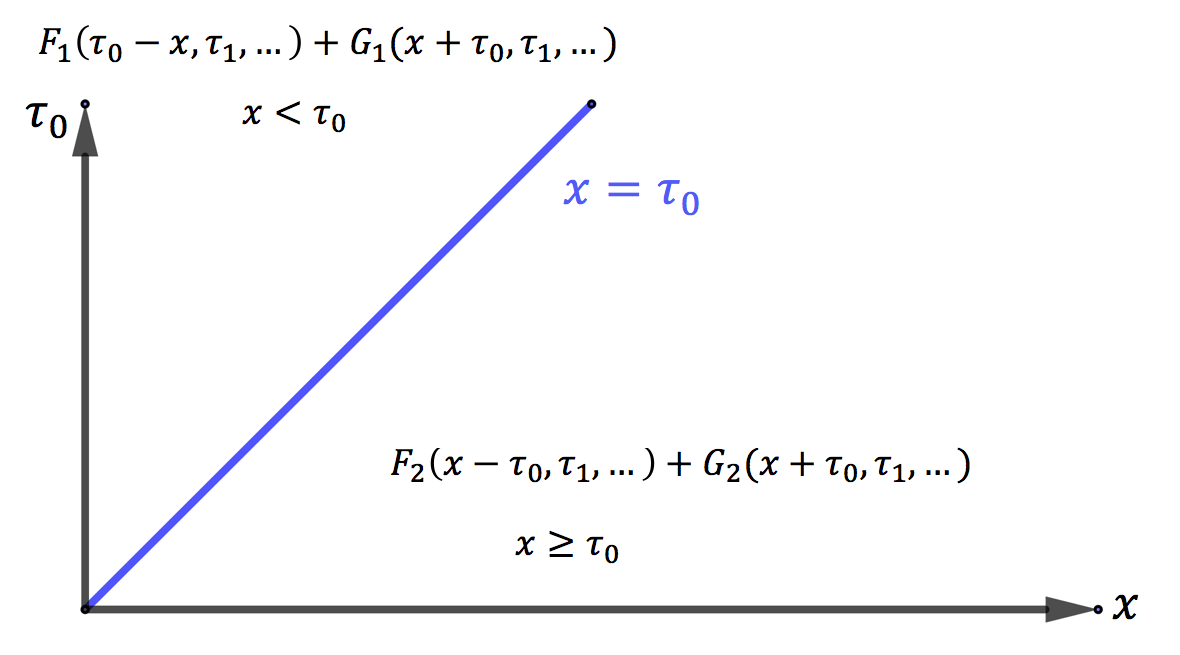
\includegraphics[scale = 0.5]{HLpic.png}
%\label{HLpic}
%\end{figure}
}
\subsubsection*{The case $x<\tau_0$}
We consider the case $x<t.$ First, we use
\begin{align*}
\eta &= \eta_0 + \epsilon \eta_1 + \mathcal{O}(\epsilon^2)  \\
&= F_1(t-x, \epsilon t, \ldots) + G_1(x+t, \epsilon t, \ldots) + \epsilon \eta_1 + \mathcal{O}(\epsilon^2) \\
&= F_1(-\xi, \tau_1, \ldots) + G_1(\zeta, \tau_1, \ldots) + \epsilon \eta_1 + \mathcal{O}(\epsilon^2) \\
&= F_1+G_1 + \epsilon \eta_1 +  \mathcal{O}(\epsilon^2).
\end{align*}
For ease of writing, we suppress explicit dependence on variables, though the reader should bear in mind that function $F_1, (G_1)$ depend on $-\xi, (\zeta), \tau_1, \tau_2,$ etc. In addition, observe that
\begin{align*}
(\partial_t^2 - \partial_x^2) = \left( - 4\partial_\xi \partial_\zeta + 2\epsilon(\partial_\zeta \partial_{\tau_1} - \partial_\xi\partial_{\tau_1}) + \epsilon^2 \partial_{\tau_1}^2 \right),
\end{align*}
so that the LHS of \eqref{srfceq0} becomes
\begin{align}
(\partial_t^2 - \partial_x^2) \eta &= \epsilon \left(- 4\eta_{1\xi \zeta} - 2\partial_{\xi}\partial_{\tau_1}(F_1)_{\tau_1} + 2\partial_\zeta \partial_{\tau_1}G_1 \right) + \mathcal{O}(\epsilon^2). \label{LHS1-1}
\end{align}
Now, we deal with the RHS of \eqref{srfceq0}. By appropriate substitutions, the terms become:
\begin{align*}
\frac{1}{3}\eta_{xxxx} &= \frac{1}{3}(\partial_\xi^4 F_1 + \partial_\zeta^4G_1+ \mathcal{O}(\epsilon)); \\
\left( \int^{x}_{0} \eta_t \D x' \right)^2 &= \left( \int^{x}_{0} \eta_{0t} \D x' \right)^2 + \mathcal{O}(\epsilon) \\
&= \left( \int^{x}_{0}(-\partial_{\xi'} + \partial_{\zeta'} + \epsilon \partial_{\tau_1}) (F_1+G_1) \D x' \right)^2 + \mathcal{O}(\epsilon)\\ 
&= \left( \int^{x}_{0} - \partial_{\xi'}F_1 + \partial_{\zeta'} G_1 \D x' \right)^2 + \mathcal{O}(\epsilon)\\
&= \left( \int^{x}_{0} -\partial_{\xi'}F_1 \D x'\right)^2 - 2\left( \int^{x}_{0}( \partial_{\xi'} F_1 \D x'\right)\left( \int^{x}_{0}\partial_{\zeta'}G_1 \D x'\right) + \left( \int^{x}_{0} \partial_{\zeta'} G_1 \D x'\right)^2 + \mathcal{O}(\epsilon) \\
&= (F_1 - F_1(\tau_0))^2 - 2(F_1 - F_1(\tau_0))(G_1 - G_1(\tau_0)) + (G_1 - G_1(\tau_0))^2 + \mathcal{O}(\epsilon),
\end{align*}
where for the last line we translate $\xi' = x'-t, \zeta' = x'+t$ to obtain
\begin{align*}
 \int^{x}_{0} -\partial_{\xi'}(F_1(\tau_0 - \xi')) \D x' &=  \int^{x-t}_{-t}(F_1)_{\xi'}(-\xi', \tau_1) \D \xi' =\int^{\xi}_{-\tau_0}(F_1)_{\xi'}(-\xi', \tau_1) \D \xi' = F_1 - F_1(\tau_0), \\
\int^{x}_{0} (G_1)_{\zeta'}(x'+\tau_0, \tau_1) \D x' &=  \int^{x+t}_{t}(G_1)_{\zeta'}(\zeta', \tau_1) \D \zeta' = \int^{\zeta}_{\tau_0}(G_1)_{\zeta'}(\zeta', \tau_1) \D \zeta' = G_1 - G_1(\tau_0).
\end{align*}
Note that previously we wrongly assumed that there is some strange term $F(-t).$ But $F$ that we used was rather $F_2,$ which is appropriate when $x \geq \tau_0.$ In this case, $x< \tau_0,$ so we need to use $F_1,$ which provides the right viewpoint. Finally, from Proposition \ref{HTtransformed}, we also have
\begin{align*}
\int_0^\infty \partial_t &\left( \eta \int^{y}_0\eta_{t} \D y' \right) \left[ \frac{1}{x-y} + \frac{1}{x+y} \right] \D y \\
&=  \int_0^{\tau_0} \left( 2 F_1  \partial_\xi F_1 + 2 G_1 \partial_\zeta G_1 \right) \left[ \frac{1}{x-y} + \frac{1}{x+y} \right] \D y +\int_{\tau_0}^\infty (2 F_2 \partial_\xi F_2 + 2 G_2 \partial_\zeta G_2 )\left[ \frac{1}{x-y} + \frac{1}{x+y} \right] \D y.
\end{align*}
Substitution of terms into the RHS of \eqref{srfceq0} leads to:
\begin{align}
\frac{1}{3} \eta_{xxxx} &+ \frac{d}{dx} \frac{1}{\pi} \int_0^\infty \partial_t \left( \eta \int^{y}_0\eta_{t} \D y' \right) \left[ \frac{1}{x-y} + \frac{1}{x+y} \right] \D y + \frac{1}{2} \partial^2_x\left(\int^{x}_0\eta_{t} \D x' \right)^2 \nonumber\\
&= \frac{1}{3}(\partial_\xi^4 F_1 + \partial_\zeta^4 G_1 + \frac{1}{\pi} (\partial_\xi + \partial_\zeta) \left( \int_0^{\tau_0} \left( 2 F_1  \partial_\xi F_1 + 2 G_1 \partial_\zeta G_1 \right) \left[ \frac{1}{x-y} + \frac{1}{x+y} \right] \D y +\int_{\tau_0}^\infty (2 F_2 \partial_\xi F_2 + 2 G_2 \partial_\zeta G_2 )\left[ \frac{1}{x-y} + \frac{1}{x+y} \right] \D y \right) \nonumber \\
&+ \frac{1}{2} (\partial_\xi^2 + 2\partial_\xi \partial_\zeta + \partial_\zeta^2) \left( (F_1 - F_1(\tau_0))^2 - 2(F_1 - F_1(\tau_0))(G_1- G_1(\tau_0)) + (G_1 - G_1(\tau_0))^2 \right) + \mathcal{O}(\epsilon) \nonumber \\
&=  \frac{1}{3}(\partial_\xi^4 F_1 + \partial_\zeta^4 G_1 + \frac{1}{\pi} (\partial_\xi + \partial_\zeta) \left( \int_0^{\tau_0} \left( 2 F_1  \partial_\xi F_1 + 2 G_1 \partial_\zeta G_1 \right) \left[ \frac{1}{x-y} + \frac{1}{x+y} \right] \D y +\int_{\tau_0}^\infty (2 F_2 \partial_\xi F_2 + 2 G_2 \partial_\zeta G_2 )\left[ \frac{1}{x-y} + \frac{1}{x+y} \right] \D y \right) \nonumber \\
&+ \partial_\xi\left( (F_1 - G_1)\partial_\xi F_1 \right)+  \partial_\zeta \left( (G_1 - F_1)\partial_\zeta G_1)\right) - 2 \partial_\xi F_1 \partial_\zeta G_1. \label{RHS1-1}
\end{align}
Combining \eqref{LHS1-1} and \eqref{RHS1-1}, in $\mathcal{O}(\epsilon^1)$ we have
\begin{equation}\label{srfceqHL2-1}
\begin{aligned}
- 4\eta_{1\xi \zeta} &= 2 \partial_\xi \partial_{\tau_1}F_1 - 2\partial_{\zeta} \partial_{\tau_1}G_1  + \frac{1}{3}(\partial_\xi^4 F_1 + \partial_\zeta^4 G_1) \\
&+ \frac{1}{\pi} (\partial_\xi + \partial_\zeta) \left( \int_0^{\tau_0} \left( 2 F_1  \partial_\xi F_1 + 2 G_1 \partial_\zeta G_1 \right) \left[ \frac{1}{x-y} + \frac{1}{x+y} \right] \D y +\int_{\tau_0}^\infty (2 F_2 \partial_\xi F_2 + 2 G_2 \partial_\zeta G_2 )\left[ \frac{1}{x-y} + \frac{1}{x+y} \right] \D y \right) \\
&+ \partial_\xi\left( (F_1 - G_1)\partial_\xi F_1 \right) +  \partial_\zeta \left( (G_1 - F_1)\partial_\zeta G_1 \right) - 2 \partial_\xi F_1 \partial_\zeta G_1.
\end{aligned}
\end{equation}
By rearranging appropriately, \eqref{srfceqHL2-1} becomes
\begin{equation}\label{srfceqHL3-1}
\begin{aligned}
- 4\eta_{1\xi \zeta} &= \partial_\xi (2 \partial_{\tau_1}F_1 + \frac{1}{3} \partial_\xi^3 F_1 + F_1\partial_\xi F_1 + \frac{1}{\pi} \left( \int_0^{\tau_0} 2 F_1  \partial_\xi F_1 \left[ \frac{1}{x-y} + \frac{1}{x+y} \right] \D y +\int_{\tau_0}^\infty 2 F_2 \partial_\xi F_2\left[ \frac{1}{x-y} + \frac{1}{x+y} \right] \D y \right))  \\
&+ \partial_\zeta(- 2 \partial_{\tau_1} G_1 +  \frac{1}{3} \partial_\zeta^3 G_1+ G_1 \partial_{\zeta} G_1  + \frac{1}{\pi} \left( \int_0^{\tau_0}  2 G_1 \partial_\zeta G_1 \left[ \frac{1}{x-y} + \frac{1}{x+y} \right] \D y +\int_{\tau_0}^\infty 2 G_2 \partial_\zeta G_2 \left[ \frac{1}{x-y} + \frac{1}{x+y} \right] \D y \right)) \\
&+ \partial_{\xi}(-G_1 \partial_\xi F_1 + \frac{1}{\pi} \left( \int_0^{\tau_0} 2 G_1 \partial_\zeta G_1 \left[ \frac{1}{x-y} + \frac{1}{x+y} \right] \D y +\int_{\tau_0}^\infty 2 G_2 \partial_\zeta G_2 \left[ \frac{1}{x-y} + \frac{1}{x+y} \right] \D y \right) ) \\
&+ \partial_{\zeta}( - F_1\partial_\zeta G_1 + \frac{1}{\pi} \left( \int_0^{\tau_0} 2 F_1  \partial_\xi F_1 \left[ \frac{1}{x-y} + \frac{1}{x+y} \right] \D y +\int_{\tau_0}^\infty 2 F_2 \partial_\xi F_2  \left[ \frac{1}{x-y} + \frac{1}{x+y} \right] \D y \right)) - 2 \partial_\xi F_1 \partial_\zeta G_1. 
\end{aligned}
\end{equation}
Integration of \eqref{srfceqHL3-1} with respect to $\zeta$ yields
\begin{equation}
\begin{aligned}
- 4\eta_{1\xi} &= \zeta \partial_\xi (2 \partial_{\tau_1}F_1 + \frac{1}{3} \partial_\xi^3 F_1 + F_1\partial_\xi F_1 + \frac{1}{\pi} \left( \int_0^{\tau_0} 2 F_1  \partial_\xi F_1 \left[ \frac{1}{x-y} + \frac{1}{x+y} \right] \D y +\int_{\tau_0}^\infty 2 F_2 \partial_\xi F_2\left[ \frac{1}{x-y} + \frac{1}{x+y} \right] \D y \right))  \\
&+(- 2 \partial_{\tau_1} G_1 +  \frac{1}{3} \partial_\zeta^3 G_1+ G_1 \partial_{\zeta} G_1  + \frac{1}{\pi} \left( \int_0^{\tau_0}  2 G_1 \partial_\zeta G_1 \left[ \frac{1}{x-y} + \frac{1}{x+y} \right] \D y +\int_{\tau_0}^\infty 2 G_2 \partial_\zeta G_2 \left[ \frac{1}{x-y} + \frac{1}{x+y} \right] \D y \right)) \\
&+ \partial_{\xi}\int (G_1 \partial_\xi F_1 + \frac{1}{\pi} \left( \int_0^{\tau_0} 2 G_1 \partial_\zeta G_1 \left[ \frac{1}{x-y} + \frac{1}{x+y} \right] \D y +\int_{\tau_0}^\infty 2 G_2 \partial_\zeta G_2 \left[ \frac{1}{x-y} + \frac{1}{x+y} \right] \D y \right) )\D \zeta \\
&+(-F_1\partial_\zeta G_1 + \frac{1}{\pi} \left( \int_0^{\tau_0} 2 F_1  \partial_\xi F_1 \left[ \frac{1}{x-y} + \frac{1}{x+y} \right] \D y +\int_{\tau_0}^\infty 2 F_2 \partial_\xi F_2  \left[ \frac{1}{x-y} + \frac{1}{x+y} \right] \D y \right)) - 2 \partial_\xi F_1 G_1. 
\end{aligned}
\end{equation}
and further integration with respect to $\xi$ leads to
\begin{align*}
- 4\eta_{1} &= \zeta (2 \partial_{\tau_1}F_1 + \frac{1}{3} \partial_\xi^3 F_1 + F_1\partial_\xi F_1 + \frac{1}{\pi} \left( \int_0^{\tau_0} 2 F_1  \partial_\xi F_1 \left[ \frac{1}{x-y} + \frac{1}{x+y} \right] \D y +\int_{\tau_0}^\infty 2 F_2 \partial_\xi F_2\left[ \frac{1}{x-y} + \frac{1}{x+y} \right] \D y \right) ) \\
&+\xi (- 2 \partial_{\tau_1} G_1 +  \frac{1}{3} \partial_\zeta^3 G_1+ G_1 \partial_{\zeta} G_1  + \frac{1}{\pi} \left( \int_0^{\tau_0}  2 G_1 \partial_\zeta G_1 \left[ \frac{1}{x-y} + \frac{1}{x+y} \right] \D y +\int_{\tau_0}^\infty 2 G_2 \partial_\zeta G_2 \left[ \frac{1}{x-y} + \frac{1}{x+y} \right] \D y \right) )\\
&+ \int (G_1 \partial_\xi F_1 + \frac{1}{\pi} \left( \int_0^{\tau_0} 2 G_1 \partial_\zeta G_1 \left[ \frac{1}{x-y} + \frac{1}{x+y} \right] \D y +\int_{\tau_0}^\infty 2 G_2 \partial_\zeta G_2 \left[ \frac{1}{x-y} + \frac{1}{x+y} \right] \D y \right) )\D \zeta \\
&+\int (-F_1\partial_\zeta G_1 + \frac{1}{\pi} \left( \int_0^{\tau_0} 2 F_1  \partial_\xi F_1 \left[ \frac{1}{x-y} + \frac{1}{x+y} \right] \D y +\int_{\tau_0}^\infty 2 F_2 \partial_\xi F_2  \left[ \frac{1}{x-y} + \frac{1}{x+y} \right] \D y \right))\D \xi - 2 F_1 G_1. 
\end{align*}
Since $\eta_1$ must be bounded, we must have 
\begin{align}
2 \partial_{\tau_1}F_1 + \frac{1}{3} \partial_\xi^3 F_1 + F_1\partial_\xi F_1 + \frac{1}{\pi} \left( \int_0^{\tau_0} 2 F_1  \partial_\xi F_1 \left[ \frac{1}{x-y} + \frac{1}{x+y} \right] \D y +\int_{\tau_0}^\infty 2 F_2 \partial_\xi F_2\left[ \frac{1}{x-y} + \frac{1}{x+y} \right] \D y \right) &= 0 \label{KdVish1}, \\
- 2 \partial_{\tau_1} G_1 +  \frac{1}{3} \partial_\zeta^3 G_1+ G_1 \partial_{\zeta} G_1  + \frac{1}{\pi} \left( \int_0^{\tau_0}  2 G_1 \partial_\zeta G_1 \left[ \frac{1}{x-y} + \frac{1}{x+y} \right] \D y +\int_{\tau_0}^\infty 2 G_2 \partial_\zeta G_2 \left[ \frac{1}{x-y} + \frac{1}{x+y} \right] \D y \right) &= 0. \label{KdVish3}
\end{align}
In other words, we have obtained two KdV-like equations, \eqref{KdVish1} and \eqref{KdVish3}, whose solutions $F_1, G_1$ describe behaviour of the surface elevation in the leading order, when $x<\tau_0.$
 
\subsubsection*{The case $x\geq \tau_0$}
On the domain $x\geq \tau_0,$ we use 
\begin{align*}
\eta &= \eta_0 + \epsilon \eta_1 + \mathcal{O}(\epsilon^2)  \\
&= F_2(x-t, \epsilon t, \ldots) + G_2(x+t, \epsilon t, \ldots) + \epsilon \eta_1 + \mathcal{O}(\epsilon^2) \\
&= F_2(\xi, \tau_1, \ldots) + G_2(\zeta, \tau_1, \ldots) + \epsilon \eta_1 + \mathcal{O}(\epsilon^2) \\
&= F_2+G_2 + \epsilon \eta_1 +  \mathcal{O}(\epsilon^2).
\end{align*}
For ease of writing, we suppress explicit dependence on variables, though the reader should bear in mind that function $F_2, (G_2)$ depend on $\xi, (\zeta), \tau_1, \tau_2,$ etc. In addition, D'Alembert operator becomes 
\begin{align*}
(\partial_t^2 - \partial_x^2) = \left( - 4\partial_\xi \partial_\zeta + 2\epsilon(\partial_\zeta \partial_{\tau_1} - \partial_\xi\partial_{\tau_1}) + \epsilon^2 \partial_{\tau_1}^2 \right),
\end{align*}
so that the LHS of \eqref{srfceq0} becomes
\begin{align}
(\partial_t^2 - \partial_x^2) \eta &= \epsilon \left(- 4\eta_{1\xi \zeta} - 2\partial_{\xi}\partial_{\tau_1} F_1 + 2\partial_{\zeta}\partial_{\tau_1}G_1\right) + \mathcal{O}(\epsilon^2). \label{LHS1-2}
\end{align}
Now, we deal with the RHS of \eqref{srfceq0}. By appropriate substitutions, the terms become:
\begin{align*}
\frac{1}{3}\eta_{xxxx} &= \frac{1}{3}(\partial_\xi^4 F_2 + \partial_\zeta^4(G_2)+ \mathcal{O}(\epsilon)); \\
\left( \int^{x}_{0} \eta_t \D x' \right)^2 &= \left( \int^{\tau_0}_{0} \eta_t \D x' + \int_{\tau_0}^{x} \eta_t \D x' \right)^2 \\
&= \left( \int^{\tau_0}_{0} \eta_{0t} \D x' + \int_{\tau_0}^{x} \eta_{0t} \D x' \right)^2 + \mathcal{O}(\epsilon) \\ 
&= \left( \int^{\tau_0}_{0} (-\partial_{\xi'} + \partial_{\zeta'} + \epsilon \partial_{\tau_1}) (F_1+G_1) \D x' + \int_{\tau_0}^{x} (-\partial_{\xi'} + \partial_{\zeta'} + \epsilon \partial_{\tau_1}) (F_2+G_2) \D x' \right)^2 + \mathcal{O}(\epsilon) \\
&= \left( \int^{\tau_0}_{0} (-\partial_{\xi'} + \partial_{\zeta'}) (F_1+G_1) \D x' + \int_{\tau_0}^{x} (-\partial_{\xi'} + \partial_{\zeta'}) (F_2+G_2) \D x' \right)^2 + \mathcal{O}(\epsilon), \\
&= F^2_2 - 2F_2 G_2 + G_2^2 + \mathcal{O}(\epsilon),
\end{align*}
where for the last line we have simplified as follows:
\begin{align*}
\int^{\tau_0}_{0} -\partial_{\xi'}(F_1(\tau_0 - \xi')) \D x' &=  -\int^{0}_{-\tau_0}\partial_{\xi'} F_1(-\xi', \tau_1) \D \xi' = -F_1(0) + F_1(\tau_0), \\
\int^{\tau_0}_{0} \partial_{\zeta'} G_1(x'+\tau_0, \tau_1) \D x' &=  \int^{2\tau_0}_{\tau_0}\partial_{\zeta'} G_1(\zeta', \tau_1) \D \zeta'  = G_1(2\tau_0) - G_1(\tau_0) \\
\int_{\tau_0}^{x} -\partial_{\xi'}(F_2(\tau_0 - \xi')) \D x' &=  -\int_{0}^{x-\tau_0}\partial_{\xi'} F_2(\xi', \tau_1) \D \xi' = -F_2 + F_2(0), \\
\int_{\tau_0}^{x} \partial_{\zeta'} G_2(x'+\tau_0, \tau_1) \D x' &=  \int_{2\tau_0}^{x+\tau_0}\partial_{\zeta'} G_2(\zeta', \tau_1) \D \zeta'  = G_2 - G_2(2\tau_0).
\end{align*}
Addition of terms yields
\begin{align*}
\int^{\tau_0}_{0} (-\partial_{\xi'} + \partial_{\zeta'}) (F_1+G_1) \D x' + \int_{\tau_0}^{x} (-\partial_{\xi'} + \partial_{\zeta'}) (F_2+G_2) \D x' &=  -F_1(0) + F_1(\tau_0) + G_1(2\tau_0) - G_1(\tau_0) -F_2 + F_2(0) + G_2 - G_2(2\tau_0) \\
&= -F_2  + G_2 -F_1(0) + F_2(0) + G_1(2\tau_0)- G_2(2\tau_0) + F_1(\tau_0)- G_1(\tau_0) \\
&=  -F_2  + G_2,
\end{align*}
where we recall the interface conditions $F_1(0) = F_2(0), G_1(2\tau_0) =G_2(2\tau_0)$ and the boundary conditions $\eta_x(0,t) = 0.$ The latter yields that
\[ \eta_x(0,t) = \partial_x(F_1(\tau_0-x) + G_1(\tau_0+x))\bigg|^{x=0} =  -F_1'(\tau_0) + G_1'(\tau_0) = 0 \implies  F_1'(\tau_0) = G_1'(\tau_0)  \implies F_1(\tau_0) = G_1(\tau_0), \]
where we set the scalar of integration to be 0. Finally, by Proposition \ref{HTtransformed}, we also have 
\begin{align*}
\int_0^\infty \partial_t &\left( \eta \int^{y}_0\eta_{t} \D y' \right) \left[ \frac{1}{x-y} + \frac{1}{x+y} \right] \D y \\
&=  \int_0^{\tau_0} \left( 2 F_1  \partial_\xi F_1 + 2 G_1 \partial_\zeta G_1 \right) \left[ \frac{1}{x-y} + \frac{1}{x+y} \right] \D y +\int_{\tau_0}^\infty (2 F_2 \partial_\xi F_2 + 2 G_2 \partial_\zeta G_2 )\left[ \frac{1}{x-y} + \frac{1}{x+y} \right] \D y.
\end{align*}
Substitution of terms into the RHS of \eqref{srfceq0} leads to:
\begin{align}
\frac{1}{3} \eta_{xxxx} &+ \frac{d}{dx} \frac{1}{\pi} \int_0^\infty \partial_t \left( \eta \int^{y}_0\eta_{t} \D y' \right) \left[ \frac{1}{x-y} + \frac{1}{x+y} \right] \D y + \frac{1}{2} \partial^2_x\left(\int^{x}_0\eta_{t} \D x' \right)^2 \nonumber\\
&= \frac{1}{3}(\partial_\xi^4 F_2 + \partial_\zeta^4 G_2 + \frac{1}{\pi} (\partial_\xi + \partial_\zeta) \left( \int_0^{\tau_0} \left( 2 F_1  \partial_\xi F_1 + 2 G_1 \partial_\zeta G_1 \right) \left[ \frac{1}{x-y} + \frac{1}{x+y} \right] \D y +\int_{\tau_0}^\infty (2 F_2 \partial_\xi F_2 + 2 G_2 \partial_\zeta G_2 )\left[ \frac{1}{x-y} + \frac{1}{x+y} \right] \D y \right) \nonumber \\
&+ \frac{1}{2} (\partial_\xi^2 + 2\partial_\xi \partial_\zeta + \partial_\zeta^2) \left( F^2_2 - 2F_2 G_2 + G_2^2 \right) + \mathcal{O}(\epsilon) \nonumber \\
&=  \frac{1}{3}(\partial_\xi^4 F_2 + \partial_\zeta^4 G_2 + \frac{1}{\pi} (\partial_\xi + \partial_\zeta) \left( \int_0^{\tau_0} \left( 2 F_1  \partial_\xi F_1 + 2 G_1 \partial_\zeta G_1 \right) \left[ \frac{1}{x-y} + \frac{1}{x+y} \right] \D y +\int_{\tau_0}^\infty (2 F_2 \partial_\xi F_2 + 2 G_2 \partial_\zeta G_2 )\left[ \frac{1}{x-y} + \frac{1}{x+y} \right] \D y \right) \nonumber \\
&+ \partial_\xi\left( (F_2 - G_2)\partial_\xi F_2 \right)+  \partial_\zeta \left( (G_2 - F_2)\partial_\zeta G_2\right) - 2 \partial_\xi F_2 \partial_\zeta G_2. \label{RHS1-2}
\end{align}
Combining \eqref{LHS1-2} and \eqref{RHS1-2}, in $\mathcal{O}(\epsilon^1)$ we have
\begin{equation}\label{srfceqHL2-2}
\begin{aligned}
- 4\eta_{1\xi \zeta} &= 2 \partial_\xi \partial_{\tau_1}F_2 - 2\partial_{\zeta} \partial_{\tau_1}G_2  + \frac{1}{3}(\partial_\xi^4 F_2 + \partial_\zeta^4 G_2) \\
&+ \frac{1}{\pi} (\partial_\xi + \partial_\zeta) \left( \int_0^{\tau_0} \left( 2 F_1  \partial_\xi F_1 + 2 G_1 \partial_\zeta G_1 \right) \left[ \frac{1}{x-y} + \frac{1}{x+y} \right] \D y +\int_{\tau_0}^\infty (2 F_2 \partial_\xi F_2 + 2 G_2 \partial_\zeta G_2 )\left[ \frac{1}{x-y} + \frac{1}{x+y} \right] \D y \right) \\
&+ \partial_\xi\left( (F_2 - G_2)\partial_\xi F_2 \right)+  \partial_\zeta \left( (G_2 - F_2)\partial_\zeta G_2\right) - 2 \partial_\xi F_2 \partial_\zeta G_2.
\end{aligned}
\end{equation}
By rearranging appropriately, \eqref{srfceqHL2-2} becomes
\begin{equation}\label{srfceqHL3-2}
\begin{aligned}
- 4\eta_{1\xi \zeta} &= \partial_\xi (2 \partial_{\tau_1}F_2 + \frac{1}{3} \partial_\xi^3 F_2 + F_2\partial_\xi F_2 + \frac{1}{\pi} \left( \int_0^{\tau_0} 2 F_1  \partial_\xi F_1 \left[ \frac{1}{x-y} + \frac{1}{x+y} \right] \D y +\int_{\tau_0}^\infty 2 F_2 \partial_\xi F_2\left[ \frac{1}{x-y} + \frac{1}{x+y} \right] \D y \right))  \\
&+ \partial_\zeta(- 2 \partial_{\tau_1} G_2 +  \frac{1}{3} \partial_\zeta^3 G_2+ G_2 \partial_{\zeta} G_2 + \frac{1}{\pi} \left( \int_0^{\tau_0}  2 G_1 \partial_\zeta G_1 \left[ \frac{1}{x-y} + \frac{1}{x+y} \right] \D y +\int_{\tau_0}^\infty 2 G_2 \partial_\zeta G_2 \left[ \frac{1}{x-y} + \frac{1}{x+y} \right] \D y \right)) \\
&+ \partial_{\xi}(-G_2 \partial_\xi F_2 + \frac{1}{\pi} \left( \int_0^{\tau_0} 2 G_1 \partial_\zeta G_1 \left[ \frac{1}{x-y} + \frac{1}{x+y} \right] \D y +\int_{\tau_0}^\infty 2 G_2 \partial_\zeta G_2 \left[ \frac{1}{x-y} + \frac{1}{x+y} \right] \D y \right) ) \\
&+ \partial_{\zeta}( - F_2\partial_\zeta G_2+ \frac{1}{\pi} \left( \int_0^{\tau_0} 2 F_1  \partial_\xi F_1 \left[ \frac{1}{x-y} + \frac{1}{x+y} \right] \D y +\int_{\tau_0}^\infty 2 F_2 \partial_\xi F_2  \left[ \frac{1}{x-y} + \frac{1}{x+y} \right] \D y \right)) - 2 \partial_\xi F_2 \partial_\zeta G_2. 
\end{aligned}
\end{equation}
Integration of \eqref{srfceqHL3-1} with respect to $\zeta$ yields
\begin{equation}
\begin{aligned}
- 4\eta_{1\xi} &= \zeta \partial_\xi (2 \partial_{\tau_1}F_2 + \frac{1}{3} \partial_\xi^3 F_2 + F_2\partial_\xi F_2 + \frac{1}{\pi} \left( \int_0^{\tau_0} 2 F_1  \partial_\xi F_1 \left[ \frac{1}{x-y} + \frac{1}{x+y} \right] \D y +\int_{\tau_0}^\infty 2 F_2 \partial_\xi F_2\left[ \frac{1}{x-y} + \frac{1}{x+y} \right] \D y \right))  \\
&+(- 2 \partial_{\tau_1} G_2 +  \frac{1}{3} \partial_\zeta^3 G_2+ G_2 \partial_{\zeta} G_2  + \frac{1}{\pi} \left( \int_0^{\tau_0}  2 G_1 \partial_\zeta G_1 \left[ \frac{1}{x-y} + \frac{1}{x+y} \right] \D y +\int_{\tau_0}^\infty 2 G_2 \partial_\zeta G_2 \left[ \frac{1}{x-y} + \frac{1}{x+y} \right] \D y \right)) \\
&+ \partial_{\xi}\int (G_2 \partial_\xi F_2 + \frac{1}{\pi} \left( \int_0^{\tau_0} 2 G_1 \partial_\zeta G_1 \left[ \frac{1}{x-y} + \frac{1}{x+y} \right] \D y +\int_{\tau_0}^\infty 2 G_2 \partial_\zeta G_2 \left[ \frac{1}{x-y} + \frac{1}{x+y} \right] \D y \right) )\D \zeta \\
&+(-F_2\partial_\zeta G_2 + \frac{1}{\pi} \left( \int_0^{\tau_0} 2 F_1  \partial_\xi F_1 \left[ \frac{1}{x-y} + \frac{1}{x+y} \right] \D y +\int_{\tau_0}^\infty 2 F_2 \partial_\xi F_2  \left[ \frac{1}{x-y} + \frac{1}{x+y} \right] \D y \right)) - 2 \partial_\xi F_2 G_2. 
\end{aligned}
\end{equation}
and further integration with respect to $\xi$ leads to
\begin{align*}
- 4\eta_{1} &= \zeta (2 \partial_{\tau_1}F_2 + \frac{1}{3} \partial_\xi^3 F_2 + F_2\partial_\xi F_2 + \frac{1}{\pi} \left( \int_0^{\tau_0} 2 F_1  \partial_\xi F_1 \left[ \frac{1}{x-y} + \frac{1}{x+y} \right] \D y +\int_{\tau_0}^\infty 2 F_2 \partial_\xi F_2\left[ \frac{1}{x-y} + \frac{1}{x+y} \right] \D y \right) ) \\
&+\xi (- 2 \partial_{\tau_1} G_2 +  \frac{1}{3} \partial_\zeta^3 G_2+ G_2 \partial_{\zeta} G_2  + \frac{1}{\pi} \left( \int_0^{\tau_0}  2 G_1 \partial_\zeta G_1 \left[ \frac{1}{x-y} + \frac{1}{x+y} \right] \D y +\int_{\tau_0}^\infty 2 G_2 \partial_\zeta G_2 \left[ \frac{1}{x-y} + \frac{1}{x+y} \right] \D y \right) )\\
&+ \int (G_2 \partial_\xi F_2 + \frac{1}{\pi} \left( \int_0^{\tau_0} 2 G_1 \partial_\zeta G_1 \left[ \frac{1}{x-y} + \frac{1}{x+y} \right] \D y +\int_{\tau_0}^\infty 2 G_2 \partial_\zeta G_2 \left[ \frac{1}{x-y} + \frac{1}{x+y} \right] \D y \right) )\D \zeta \\
&+\int (-F_2\partial_\zeta G_2 + \frac{1}{\pi} \left( \int_0^{\tau_0} 2 F_1  \partial_\xi F_1 \left[ \frac{1}{x-y} + \frac{1}{x+y} \right] \D y +\int_{\tau_0}^\infty 2 F_2 \partial_\xi F_2  \left[ \frac{1}{x-y} + \frac{1}{x+y} \right] \D y \right))\D \xi - 2 F_2 G_2. 
\end{align*}
Since $\eta_1$ must be bounded, we must have 
\begin{align}
2 \partial_{\tau_1}F_2 + \frac{1}{3} \partial_\xi^3 F_2 + F_2\partial_\xi F_2 + \frac{1}{\pi} \left( \int_0^{\tau_0} 2 F_1  \partial_\xi F_1 \left[ \frac{1}{x-y} + \frac{1}{x+y} \right] \D y +\int_{\tau_0}^\infty 2 F_2 \partial_\xi F_2\left[ \frac{1}{x-y} + \frac{1}{x+y} \right] \D y \right) &= 0 \label{KdVish2}, \\
- 2 \partial_{\tau_1} G_2 +  \frac{1}{3} \partial_\zeta^3 G_2+ G_2 \partial_{\zeta} G_2  + \frac{1}{\pi} \left( \int_0^{\tau_0}  2 G_1 \partial_\zeta G_1 \left[ \frac{1}{x-y} + \frac{1}{x+y} \right] \D y +\int_{\tau_0}^\infty 2 G_2 \partial_\zeta G_2 \left[ \frac{1}{x-y} + \frac{1}{x+y} \right] \D y \right) &= 0. \label{KdVish4}
\end{align}
In other words, we have obtained two KdV-like equations, \eqref{KdVish2} and \eqref{KdVish4}, whose solutions $F_2, G_2$ describe behaviour of the surface elevation in the leading order, when $x\geq \tau_0.$

\subsubsection*{Conclusion}
In summary, we have obtained 2 systems of 2 equations: one in $F_1, F_2:$
\begin{equation}\label{HLSystemF}
\begin{aligned}
2 \partial_{\tau_1}F_1 + \frac{1}{3} \partial_\xi^3 F_1 + F_1\partial_\xi F_1 + \frac{1}{\pi} \left( \int_0^{\tau_0} 2 F_1  \partial_\xi F_1 \left[ \frac{1}{x-y} + \frac{1}{x+y} \right] \D y +\int_{\tau_0}^\infty 2 F_2 \partial_\xi F_2\left[ \frac{1}{x-y} + \frac{1}{x+y} \right] \D y \right) &= 0; \\
2 \partial_{\tau_1}F_2 + \frac{1}{3} \partial_\xi^3 F_2 + F_2\partial_\xi F_2 + \frac{1}{\pi} \left( \int_0^{\tau_0} 2 F_1  \partial_\xi F_1 \left[ \frac{1}{x-y} + \frac{1}{x+y} \right] \D y +\int_{\tau_0}^\infty 2 F_2 \partial_\xi F_2\left[ \frac{1}{x-y} + \frac{1}{x+y} \right] \D y \right) &= 0,
\end{aligned}
\end{equation}
and another one in $G_1, G_2:$
\begin{equation}\label{HLSystemG}
\begin{aligned}
- 2 \partial_{\tau_1} G_1 +  \frac{1}{3} \partial_\zeta^3 G_1+ G_1 \partial_{\zeta} G_1  + \frac{1}{\pi} \left( \int_0^{\tau_0}  2 G_1 \partial_\zeta G_1 \left[ \frac{1}{x-y} + \frac{1}{x+y} \right] \D y +\int_{\tau_0}^\infty 2 G_2 \partial_\zeta G_2 \left[ \frac{1}{x-y} + \frac{1}{x+y} \right] \D y \right) &= 0; \\
- 2 \partial_{\tau_1} G_2 +  \frac{1}{3} \partial_\zeta^3 G_2+ G_2 \partial_{\zeta} G_2  + \frac{1}{\pi} \left( \int_0^{\tau_0}  2 G_1 \partial_\zeta G_1 \left[ \frac{1}{x-y} + \frac{1}{x+y} \right] \D y +\int_{\tau_0}^\infty 2 G_2 \partial_\zeta G_2 \left[ \frac{1}{x-y} + \frac{1}{x+y} \right] \D y \right) &= 0.
\end{aligned}
\end{equation}
It should be noted that even though two systems \eqref{HLSystemF} and \eqref{HLSystemG} seem to be unrelated, this separation was due to the boundary conditions that we imposed at the interface
\[ F_1(0) = F_2(0), G_1(2\tau_0) =G_2(2\tau_0), \]
and the free boundary condition at the midpoint
\[ \eta_x(0,t) = -F_1'(\tau_0)+ G_1'(\tau_0) = 0. \]
\subsubsection*{The Hilbert Transform term}
\begin{prop}\label{HTtransformed}
We have 
\begin{align*}
\int_0^\infty \partial_t &\left( \eta \int^{y}_0\eta_{t} \D y' \right) \left[ \frac{1}{x-y} + \frac{1}{x+y} \right] \D y \\
&=  \int_0^{\tau_0} \left( 2 F_1  \partial_\xi F_1 + 2 G_1 \partial_\zeta G_1 \right) \left[ \frac{1}{x-y} + \frac{1}{x+y} \right] \D y +\int_{\tau_0}^\infty (2 F_2 \partial_\xi F_2 + 2 G_2 \partial_\zeta G_2 )\left[ \frac{1}{x-y} + \frac{1}{x+y} \right] \D y.
\end{align*}
\end{prop}
\begin{proof}
Note:
\begin{align*}
\int_0^\infty \partial_t \left( \eta \int^{y}_0\eta_{t} \D y' \right) \left[ \frac{1}{x-y} + \frac{1}{x+y} \right] \D y &= \int_0^\infty (- \partial_\xi + \partial_\zeta + \epsilon \partial_{\tau_1})\left( (\eta_0 + \epsilon \eta_1) \int^{y}_0(\eta_0 + \epsilon \eta_1)_{t} \D y' \right) \left[ \frac{1}{x-y} + \frac{1}{x+y} \right] \D y + \mathcal{O}(\epsilon^2)\\
&= \int_0^\infty (- \partial_\xi + \partial_\zeta)\left( (\eta_0 + \epsilon \eta_1) \int^{y}_0(\eta_0 + \epsilon \eta_1)_{t} \D y' \right) \left[ \frac{1}{x-y} + \frac{1}{x+y} \right] \D y + \mathcal{O}(\epsilon)\\
&= \int_0^\infty (- \partial_\xi + \partial_\zeta)\left( \eta_0 \int^{y}_0 (\eta_0)_{t} \D y' \right) \left[ \frac{1}{x-y} + \frac{1}{x+y} \right] \D y + \mathcal{O}(\epsilon)\\
&= \int_0^\infty (- \partial_\xi + \partial_\zeta)\left( \eta_0 \int^{y}_0 (- \partial_\xi + \partial_\zeta + \epsilon \partial_{\tau_1})\eta_0 \D y' \right) \left[ \frac{1}{x-y} + \frac{1}{x+y} \right] \D y + \mathcal{O}(\epsilon)\\
&= \int_0^\infty (- \partial_\xi + \partial_\zeta)\left( \eta_0 \int^{y}_0 (- \partial_\xi + \partial_\zeta)\eta_0 \D y' \right) \left[ \frac{1}{x-y} + \frac{1}{x+y} \right] \D y + \mathcal{O}(\epsilon).
\end{align*}
Now, recalling that $\eta_0$ is piecewise, we split the integral:
\begin{equation}\label{Int1}
\int_0^{\tau_0} (- \partial_\xi + \partial_\zeta)\left( \eta_0 \int^{y}_0 (- \partial_\xi + \partial_\zeta)\eta_0 \D y' \right) \left[ \frac{1}{x-y} + \frac{1}{x+y} \right] \D y,
\end{equation}
and
\begin{equation}\label{Int2}
\int_{\tau_0}^\infty (- \partial_\xi + \partial_\zeta)\left( \eta_0 \int^{y}_0 (- \partial_\xi + \partial_\zeta)\eta_0 \D y' \right) \left[ \frac{1}{x-y} + \frac{1}{x+y} \right] \D y.
\end{equation}
We deal with \eqref{Int1}:
\begin{align*}
\int_0^{\tau_0} (- \partial_\xi + \partial_\zeta)\left( \eta_0 \int^{y}_0 (- \partial_\xi + \partial_\zeta)\eta_0 \D y' \right) \left[ \frac{1}{x-y} + \frac{1}{x+y} \right] \D y &= 
\int_0^{\tau_0} (- \partial_\xi + \partial_\zeta)\left( (F_1 + G_1) \int^{y}_0 (- \partial_\xi + \partial_\zeta)(F_1 + G_1) \D y' \right) \left[ \frac{1}{x-y} + \frac{1}{x+y} \right] \D y \\
&= \int_0^{\tau_0} (- \partial_\xi + \partial_\zeta)\left( (F_1 + G_1) \int^{y}_0 (-\partial_\xi F_1 + \partial_\zeta G_1) \D y' \right) \left[ \frac{1}{x-y} + \frac{1}{x+y} \right] \D y \\
&= \int_0^{\tau_0} (- \partial_\xi + \partial_\zeta)\left( (F_1 + G_1) (- (F_1-F_1(\tau_0)) + G_1 - G_1(\tau_0) )\right) \left[ \frac{1}{x-y} + \frac{1}{x+y} \right] \D y \\
&= \int_0^{\tau_0} (- \partial_\xi + \partial_\zeta)\left( (F_1 + G_1) ( - F_1 + G_1 + F_1(\tau_0) ) - G_1(\tau_0) )\right) \left[ \frac{1}{x-y} + \frac{1}{x+y} \right] \D y \\
&= \int_0^{\tau_0} \left(- \partial_\xi + \partial_\zeta) (-F_1^2 + G_1^2)  + (- \partial_\xi + \partial_\zeta)(F_1 + G_1) (F_1(\tau_0) ) - G_1(\tau_0) )\right) \left[ \frac{1}{x-y} + \frac{1}{x+y} \right] \D y \\
&= \int_0^{\tau_0} \left( 2 F_1  \partial_\xi F_1 + 2 G_1 \partial_\zeta G_1 \right) \left[ \frac{1}{x-y} + \frac{1}{x+y} \right] \D y, 
\end{align*}
where we can set $F_1(\tau_0) ) - G_1(\tau_0)  = 0$ by imposing a free end condition $\eta_x(0,t) = 0.$ Now, we deal with \eqref{Int2}:
\begin{align*}
\int_{\tau_0}^\infty (- \partial_\xi + \partial_\zeta)&\left( \eta_0 \int^{y}_0 (- \partial_\xi + \partial_\zeta)\eta_0 \D y' \right) \left[ \frac{1}{x-y} + \frac{1}{x+y} \right] \D y \\
&= \int_{\tau_0}^\infty  (- \partial_\xi + \partial_\zeta)\left( (F_2 + G_2) \left (\int^{\tau_0}_0 (- \partial_\xi + \partial_\zeta)(F_1 + G_1) \D y'  +  \int^{y}_{\tau_0} (- \partial_\xi + \partial_\zeta)(F_2 + G_2) \D y' \right) \right) \left[ \frac{1}{x-y} + \frac{1}{x+y} \right] \D y \\
&=  \int_{\tau_0}^\infty  (- \partial_\xi + \partial_\zeta)\left( (F_2 + G_2) \left( (- F_1(0) + F_1(\tau_0) + G_1(2\tau_0) - G_1(\tau_0)-  F_2 + F_2(0) + G_2 - G_2(2\tau_0) \right) \right) \left[ \frac{1}{x-y} + \frac{1}{x+y} \right] \D y \\
&=  \int_{\tau_0}^\infty  (- \partial_\xi + \partial_\zeta)\left( (F_2 + G_2) \left( - F_2 + G_2 + F_2(0) - F_1(0)  + F_1(\tau_0)  + G_1(2\tau_0) - G_2(2\tau_0) - G_1(\tau_0) \right) \right) \left[ \frac{1}{x-y} + \frac{1}{x+y} \right] \D y \\
&=  \int_{\tau_0}^\infty  (- \partial_\xi + \partial_\zeta)\left( (F_2 + G_2) (- F_2 + G_2) \right) +  (- \partial_\xi + \partial_\zeta)\left( (F_2 + G_2) (F_2(0) - F_1(0)  + F_1(\tau_0)  + G_1(2\tau_0) - G_2(2\tau_0) - G_1(\tau_0) ) \right) \left[ \frac{1}{x-y} + \frac{1}{x+y} \right] \D y.
\end{align*}
where for the last line we translate $\xi' = x'-t, \zeta' = x'+t$ to obtain
\begin{align*}
 \int^{y}_{t} -\partial_{\xi'}(F_2(\xi' - \tau_0 )) \D x' &=  \int^{y-t}_{0}(F_2)_{\xi'}(\xi', \tau_1) \D \xi' =\int^{\xi}_{0}(F_2)_{\xi'}(\xi', \tau_1) \D \xi' = F_2(\xi, \tau_1) - F_2(0, \tau_1), \\
\int^{y}_{t} \partial_{\zeta'}(G_2)(\xi'+\tau_0, \tau_1) \D x' &=  \int^{y+t}_{2t}(G_2)_{\zeta'}(\zeta', \tau_1) \D \zeta' = \int^{\zeta}_{2\tau_0}(G_2)_{\zeta'}(\zeta', \tau_1) \D \zeta' = G_2(\zeta, \tau_1) - G_2(2\tau_0, \tau_1).
\end{align*}
We have that 
\begin{align*}
\int_{\tau_0}^\infty  (- \partial_\xi + \partial_\zeta)\left( (F_2 + G_2) (- F_2 + G_2) \right) \left[ \frac{1}{x-y} + \frac{1}{x+y} \right] \D y &= \int_{\tau_0}^\infty  (- \partial_\xi + \partial_\zeta)(-F_2^2 + G_2^2)\left[ \frac{1}{x-y} + \frac{1}{x+y} \right] \D y \\
&= \int_{\tau_0}^\infty (\partial_\xi (F_2^2) + \partial_\zeta(G_2^2) )\left[ \frac{1}{x-y} + \frac{1}{x+y} \right] \D y \\
&= \int_{\tau_0}^\infty (2 F_2 \partial_\xi F_2 + 2 G_2 \partial_\zeta G_2 )\left[ \frac{1}{x-y} + \frac{1}{x+y} \right] \D y.
\end{align*}
Looking at the term
\begin{equation}\label{ConstTerm2}
 \int_{\tau_0}^\infty (- \partial_\xi + \partial_\zeta)\left( (F_2 + G_2) (F_2(0) - F_1(0)  + F_1(\tau_0)  + G_1(2\tau_0) - G_2(2\tau_0) - G_1(\tau_0) ) \right) \left[ \frac{1}{x-y} + \frac{1}{x+y} \right] \D y,
\end{equation}
we observe interaction between $F_i, G_i$ at the interface $x= \tau_0.$ If we impose continuity, then $F_2(0) = F_1(0), G_2(2\tau_0) = G_1(2\tau_0),$ which leaves us with $F_1(\tau_0)- G_1(\tau_0).$ As before, we can eliminate this term by imposing a free end condition $\eta_x(0,t) = 0.$ Therefore, the term \eqref{ConstTerm2} vanishes due to boundary conditions. So, we obtain
\begin{align*} 
\int_{\tau_0}^\infty (- \partial_\xi + \partial_\zeta)\left( \eta_0 \int^{y}_0 (- \partial_\xi + \partial_\zeta)\eta_0 \D y' \right) \left[ \frac{1}{x-y} + \frac{1}{x+y} \right] \D y &= \int_{\tau_0}^\infty  (- \partial_\xi + \partial_\zeta)\left( (F_2 + G_2) (- F_2 + G_2) \right) \left[ \frac{1}{x-y} + \frac{1}{x+y} \right] \D y \\
&= \int_{\tau_0}^\infty (2 F_2 \partial_\xi F_2 + 2 G_2 \partial_\zeta G_2 )\left[ \frac{1}{x-y} + \frac{1}{x+y} \right] \D y,
\end{align*}
so that 
\begin{align*}
\int_0^\infty \partial_t \left( \eta \int^{y}_0\eta_{t} \D y' \right) &\left[ \frac{1}{x-y} + \frac{1}{x+y} \right] \D y \\
&= \int_0^{\tau_0} (- \partial_\xi + \partial_\zeta)\left( \eta_0 \int^{y}_0 (- \partial_\xi + \partial_\zeta)\eta_0 \D y' \right) \left[ \frac{1}{x-y} + \frac{1}{x+y} \right] \D y + \int_{\tau_0}^\infty (- \partial_\xi + \partial_\zeta)\left( \eta_0 \int^{y}_0 (- \partial_\xi + \partial_\zeta)\eta_0 \D y' \right) \left[ \frac{1}{x-y} + \frac{1}{x+y} \right] \D y\\
&= \int_0^{\tau_0} \left( 2 F_1  \partial_\xi F_1 + 2 G_1 \partial_\zeta G_1 \right) \left[ \frac{1}{x-y} + \frac{1}{x+y} \right] \D y +\int_{\tau_0}^\infty (2 F_2 \partial_\xi F_2 + 2 G_2 \partial_\zeta G_2 )\left[ \frac{1}{x-y} + \frac{1}{x+y} \right] \D y.
\end{align*}
The proof is complete. 
\end{proof}

{\small\bibliography{references}}

\end{document}
